\documentclass[12pt,a4paper]{article}
\usepackage{enumerate} %item
\usepackage{CJKutf8} %chinese
\usepackage{graphicx} %insert figure
\usepackage{amsmath}
\usepackage{caption}
\usepackage{subcaption}
\usepackage{float}
\usepackage{indentfirst}
\title{Introduction to Neural Networks \\ Homework \#2-2}
\author{機械所 \\張元睿 \\N16054629}
\date{\today}

\begin{document}

	\begin{CJK}{UTF8}{bsmi}
	\maketitle
	\newpage
	
	\begin{enumerate}
	 \item Iris
		 \begin{enumerate}
			 \begin{table}[H]
			 	\caption{parameters of iris} % title of Table
			 	\centering % used for centering table
			 	\begin{tabular}{c c c c c} % centered columns (4 columns)
			 		\hline\hline %inserts double horizontal lines
			 		  & Epoch & Learning rate & first hidden & second hidden \\ [0.5ex] % inserts table
			 		%heading
			 		\hline % inserts single horizontal line
			 		HW2 & 20 & 0.1 & 2 & 3\\ % inserting body of the table
			 		toolbox & N/A & 0.0015 & 2 & 3\\
			 		 [0.5ex] % [1ex] adds vertical space
			 		\hline %inserts single line
			 	\end{tabular}
			 	\label{table:nonlin} % is used to refer this table in the text
			 \end{table}

			 \item results from HW2 
			 \\
			 \begin{figure}[H]
				\centering
				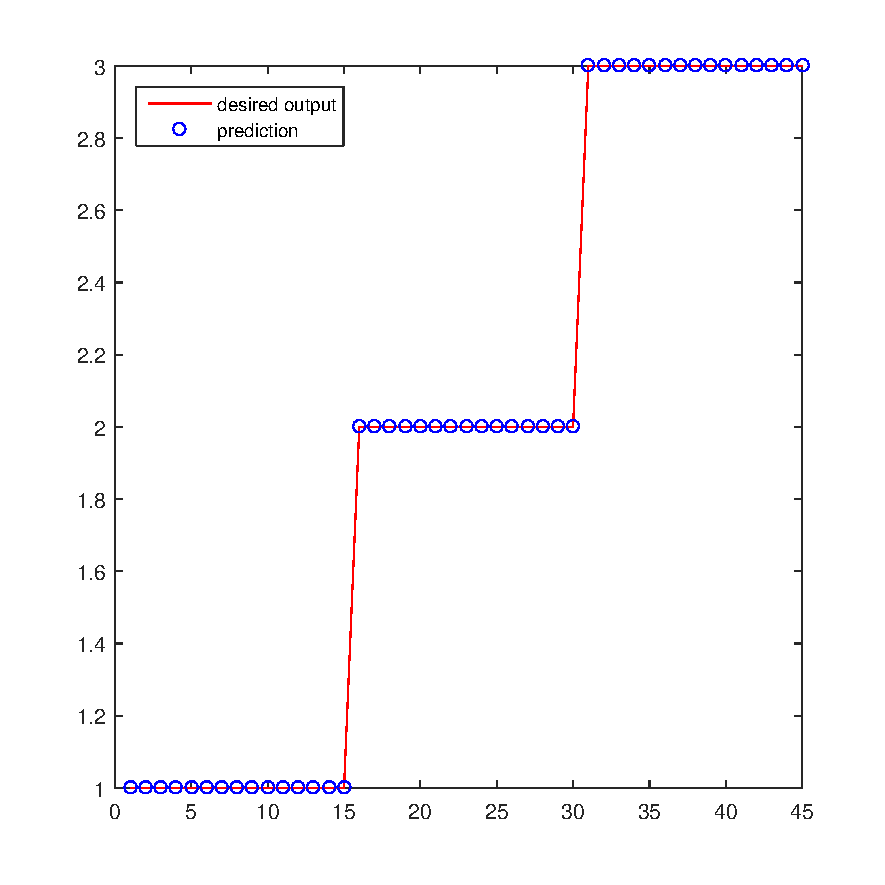
\includegraphics[scale=0.6]{irishs1}
				\caption{accuracy: 100\%} 
			 \end{figure}
		 \newpage
			 \item results from toolbox 
			 \\
			 	
		 	\begin{figure}[H]
		 		\centering
		 		\begin{subfigure}{.5\textwidth}
		 			\centering
		 			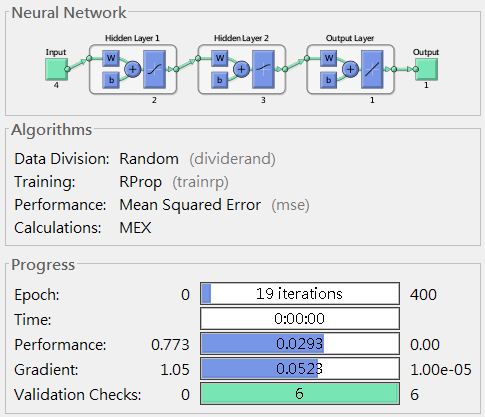
\includegraphics[width=0.92\linewidth]{RP1}
		 			\caption{RP}
		 		
		 		\end{subfigure}%
		 		\begin{subfigure}{.5\textwidth}
		 			\centering
		 			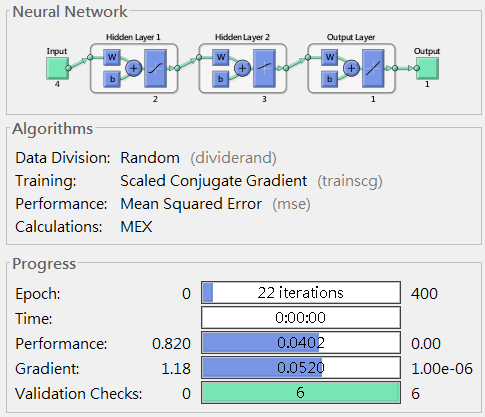
\includegraphics[width=0.92\linewidth]{SCG1}
		 			\caption{SCG}
		 		
		 		\end{subfigure}
		 		\caption{Sturctures \& Parameters}
		 		
		 	\end{figure}


		\begin{figure}[H]
			\centering
			\begin{subfigure}{.5\textwidth}
				\centering
				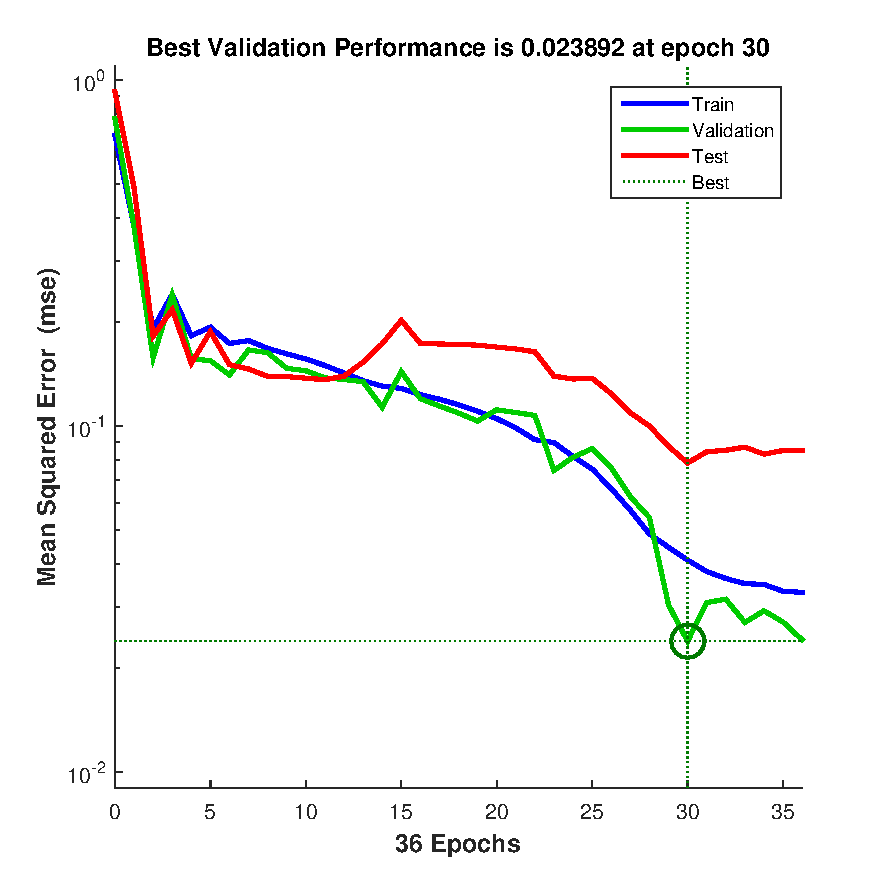
\includegraphics[width=1\linewidth]{iris_rp_per}
				\caption{RP}
				
			\end{subfigure}%
			\begin{subfigure}{.5\textwidth}
				\centering
				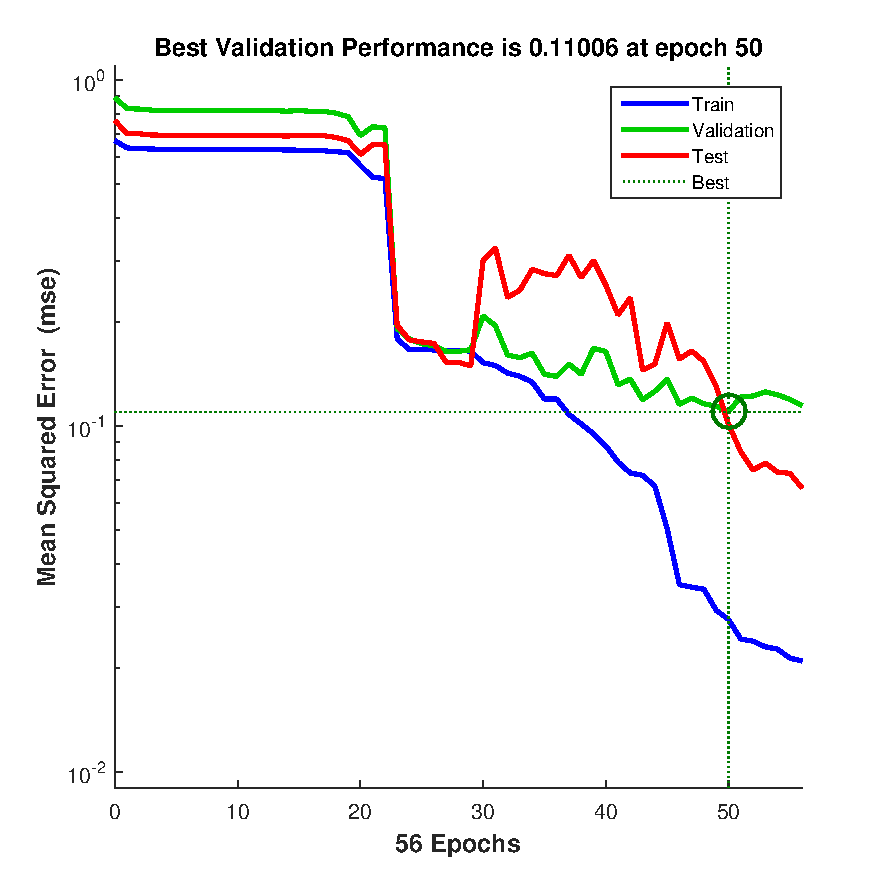
\includegraphics[width=1\linewidth]{iris_scg_per}
				\caption{SCG}
				
			\end{subfigure}
			\caption{performance}
			
		\end{figure}
	
		\begin{figure}[H]
		\centering
		\begin{subfigure}{.5\textwidth}
			\centering
			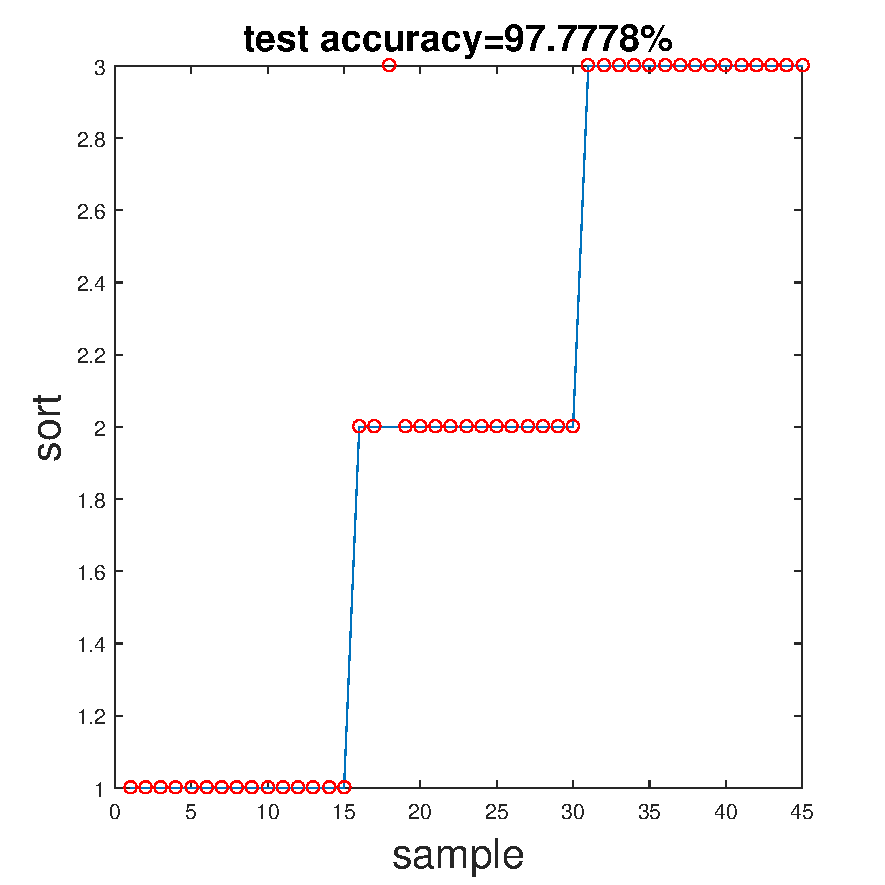
\includegraphics[width=1.05\linewidth]{iris_rp}
			\caption{RP}
			
		\end{subfigure}%
		\begin{subfigure}{.5\textwidth}
			\centering
			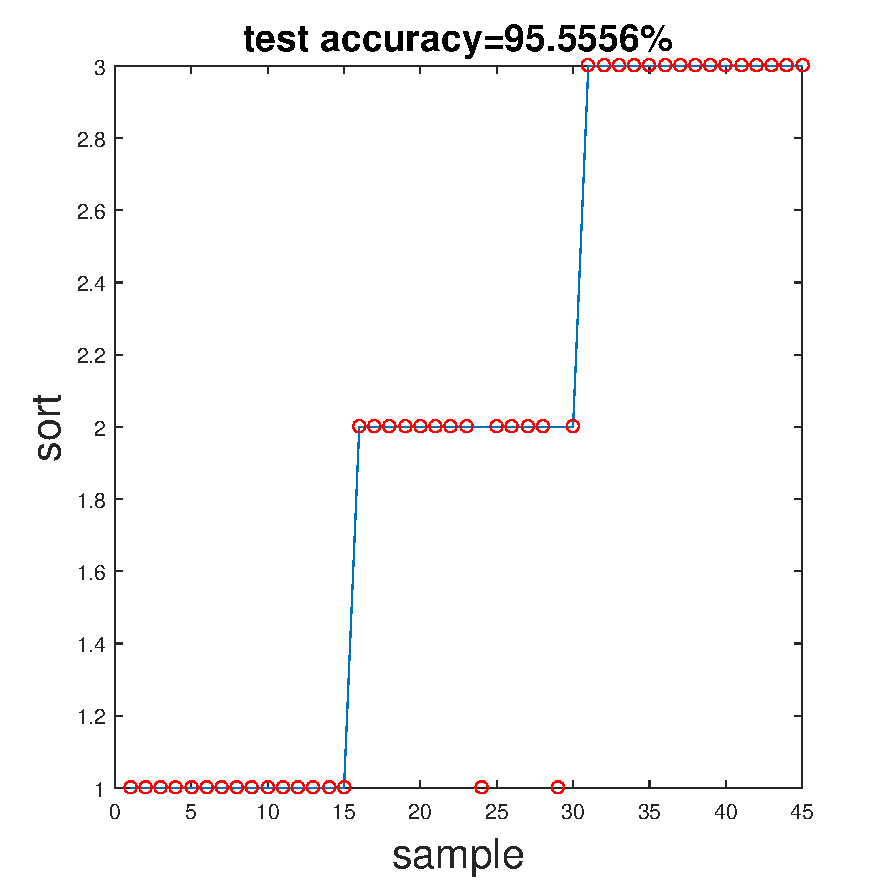
\includegraphics[width=1.05\linewidth]{iris_scg}
			\caption{SCG}
			
		\end{subfigure}
		\caption{accuracy}
		
		\end{figure}
	
		\begin{table}[H]
			\caption{accuracy of two algorithm} % title of Table
			\centering % used for centering table
			\begin{tabular}{c c c c c c c} % centered columns (4 columns)
				\hline\hline %inserts double horizontal lines
				algorithm & test1 & test2 & test3 & test4 &test5 & average\\ [0.5ex] % inserts table
				%heading
				\hline % inserts single horizontal line
				RP & 97.78\% & 100\% & 97.78\% & 97.78\% & 95.56\% & 97.78\%\\ % inserting body of the table
				SCG & 97.78\% & 95.56\% & 100\% & 100\% &97.78\% &98.22\%\\
				[0.5ex] % [1ex] adds vertical space
				\hline %inserts single line
			\end{tabular}
		\end{table}

		 \end{enumerate}
	 \newpage
	 
	 %% wine
	 \item Wine
	  \begin{enumerate}
	 	\begin{table}[H]
	 		\caption{parameters of wine} % title of Table
	 		\centering % used for centering table
	 		\begin{tabular}{c c c c c} % centered columns (4 columns)
	 			\hline\hline %inserts double horizontal lines
	 			& Epoch & Learning rate & first hidden & second hidden \\ [0.5ex] % inserts table
	 			%heading
	 			\hline % inserts single horizontal line
	 			HW2 & 30 & 0.1 & 4 & 2\\ % inserting body of the table
	 			toolbox & N/A & 0.0015 & 4 & 2\\
	 			[0.5ex] % [1ex] adds vertical space
	 			\hline %inserts single line
	 		\end{tabular}
	 		\label{table:nonlin} % is used to refer this table in the text
	 	\end{table}

	 	\item results from HW2 
	 	\\
	 	\begin{figure}[H]
	 		\centering
	 		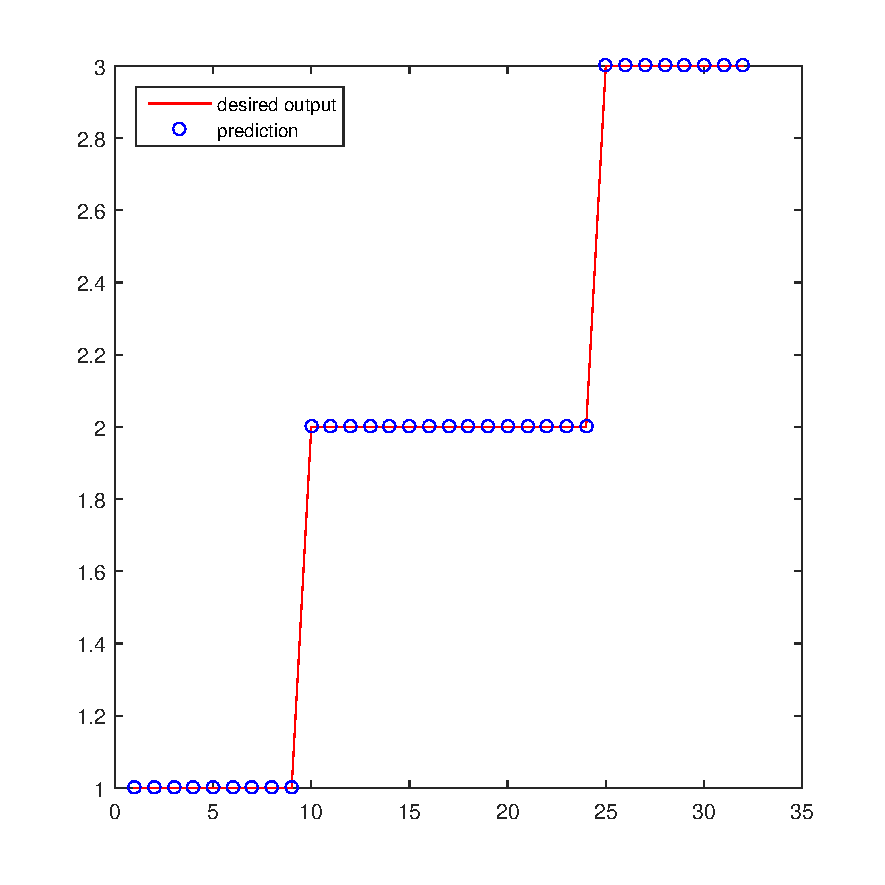
\includegraphics[scale=0.6]{winehs1}
	 		\caption{accuracy: 100\%} 
	 	\end{figure}
	 	\newpage
	 	\item results from toolbox 
	 	\\
	 	
	 	\begin{figure}[H]
	 		\centering
	 		\begin{subfigure}{.5\textwidth}
	 			\centering
	 			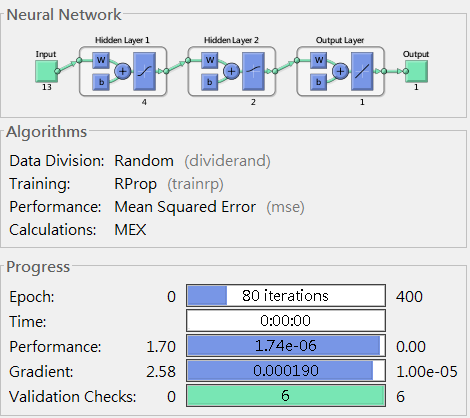
\includegraphics[width=0.92\linewidth]{RP2}
	 			\caption{RP}
	 			
	 		\end{subfigure}%
	 		\begin{subfigure}{.5\textwidth}
	 			\centering
	 			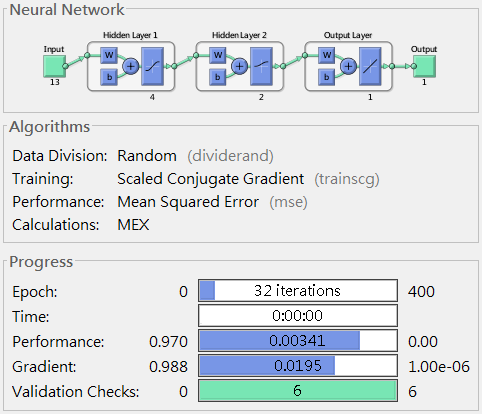
\includegraphics[width=0.92\linewidth]{SCG2}
	 			\caption{SCG}
	 			
	 		\end{subfigure}
	 		\caption{Sturctures \& Parameters}
	 		
	 	\end{figure}
	 	
	 	
	 	\begin{figure}[H]
	 		\centering
	 		\begin{subfigure}{.5\textwidth}
	 			\centering
	 			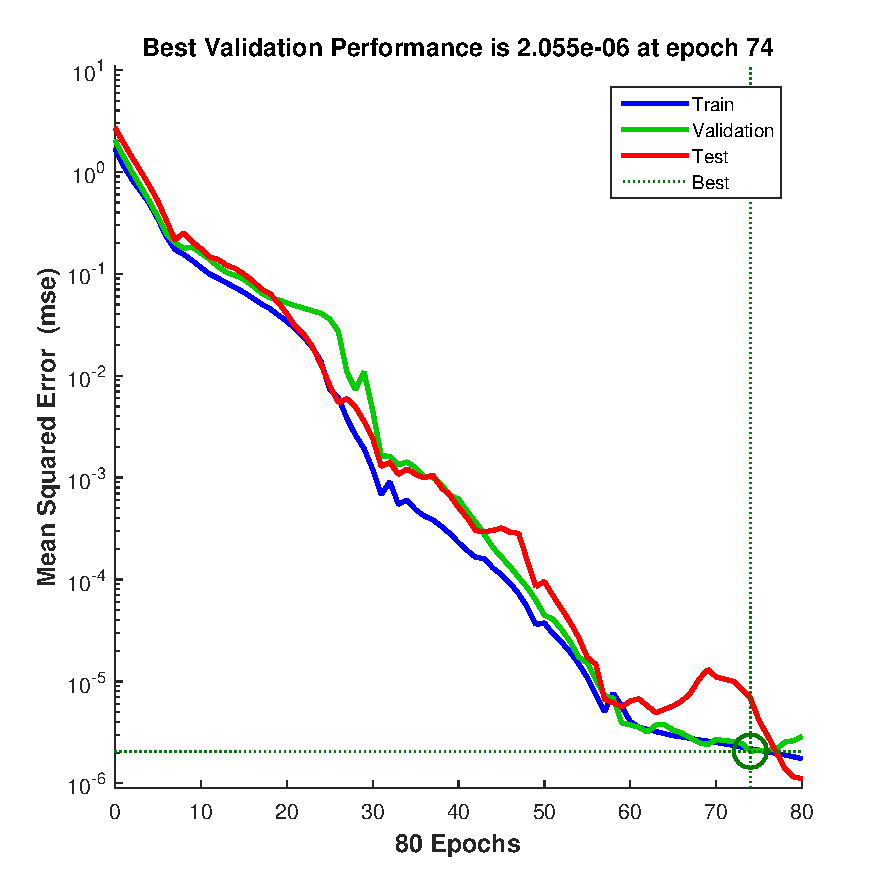
\includegraphics[width=1\linewidth]{wine_rp_per}
	 			\caption{RP}
	 			
	 		\end{subfigure}%
	 		\begin{subfigure}{.5\textwidth}
	 			\centering
	 			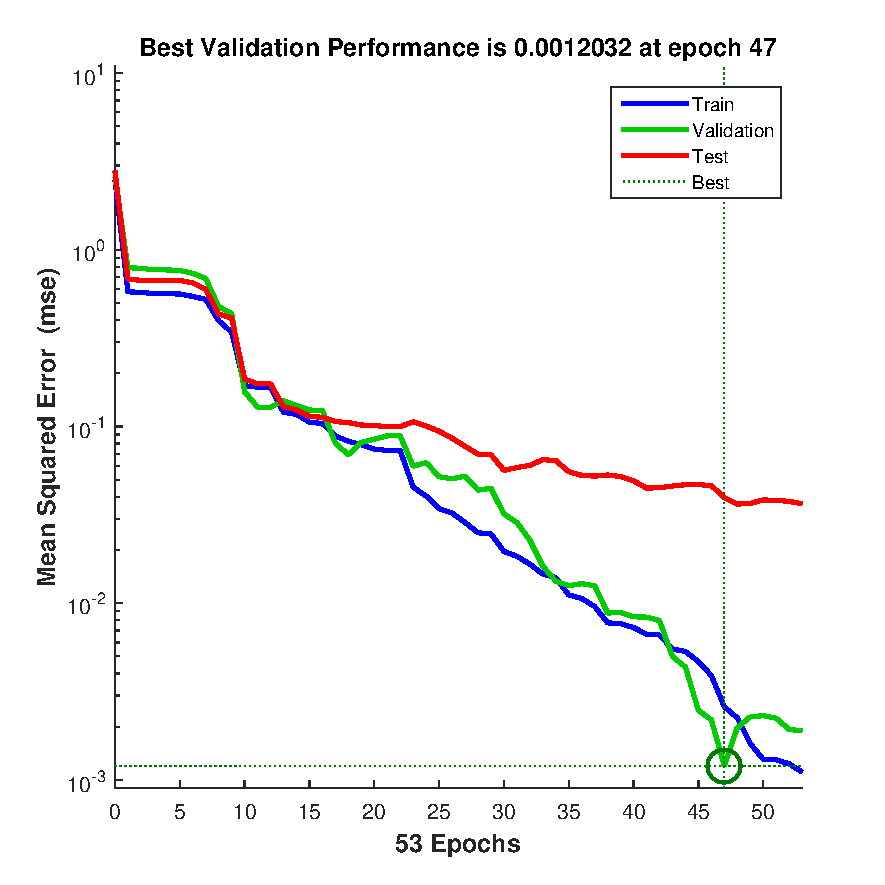
\includegraphics[width=1\linewidth]{wine_scg_per}
	 			\caption{SCG}
	 			
	 		\end{subfigure}
	 		\caption{performance}
	 		
	 	\end{figure}
	 	
	 	\begin{figure}[H]
	 		\centering
	 		\begin{subfigure}{.5\textwidth}
	 			\centering
	 			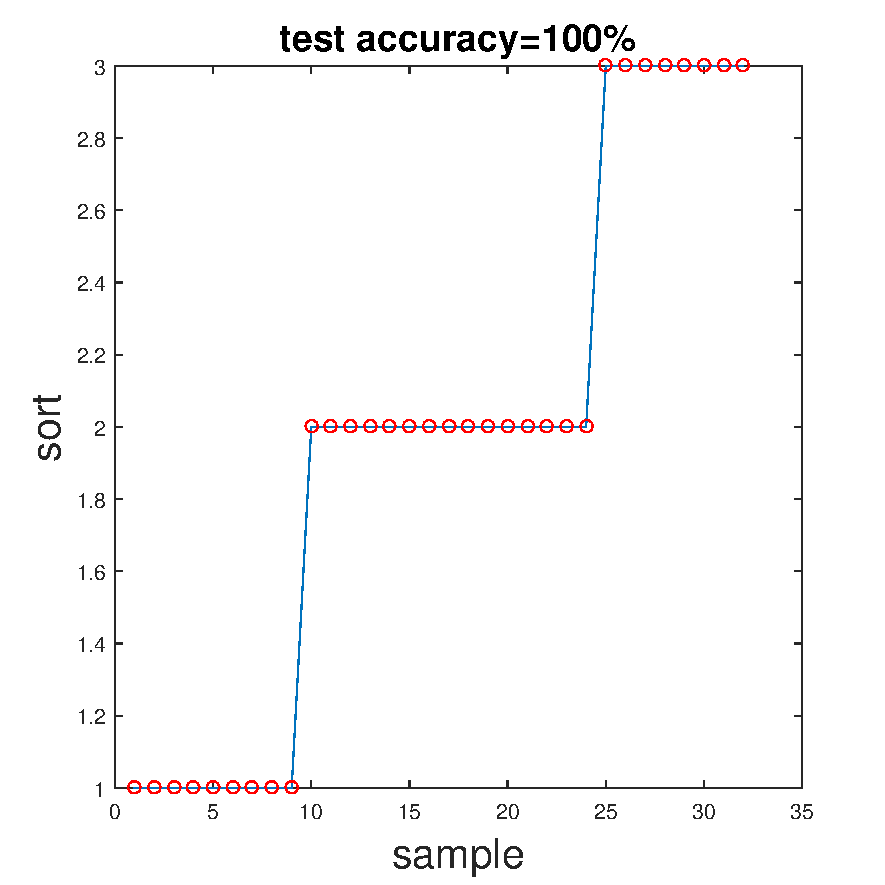
\includegraphics[width=1.05\linewidth]{wine_rp}
	 			\caption{RP}
	 			
	 		\end{subfigure}%
	 		\begin{subfigure}{.5\textwidth}
	 			\centering
	 			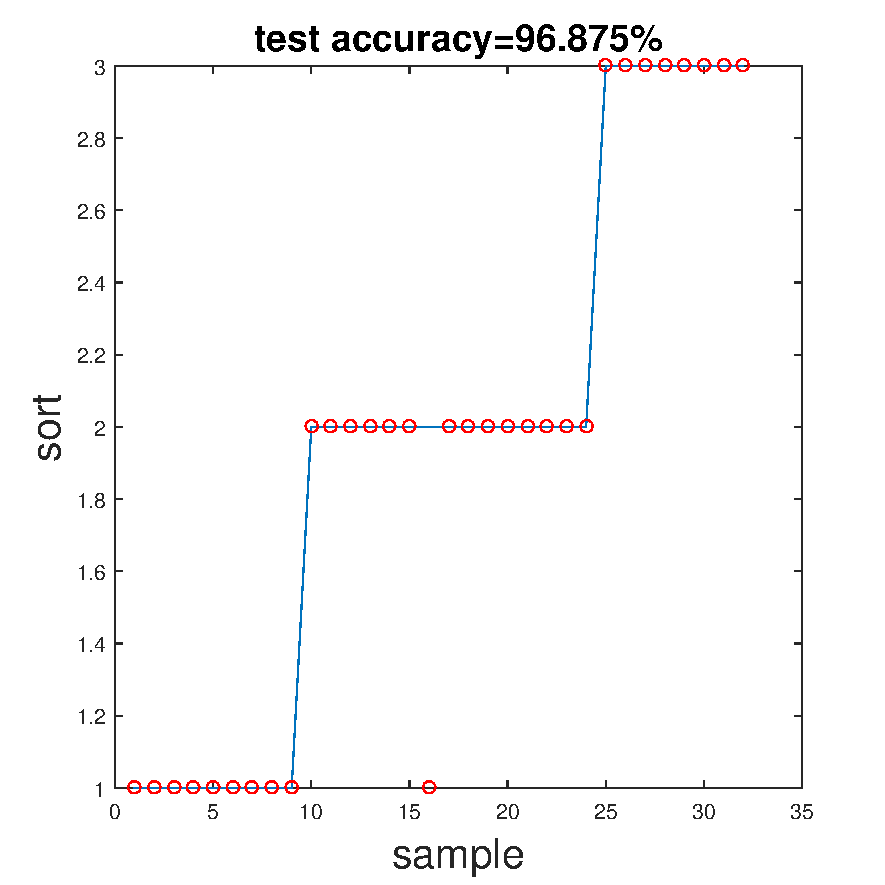
\includegraphics[width=1.05\linewidth]{wine_scg}
	 			\caption{SCG}
	 			
	 		\end{subfigure}
	 		\caption{accuracy}
	 		
	 	\end{figure}
	 	
	 	\begin{table}[H]
	 		\caption{accuracy of two algorithm} % title of Table
	 		\centering % used for centering table
	 		\begin{tabular}{c c c c c c c} % centered columns (4 columns)
	 			\hline\hline %inserts double horizontal lines
	 			algorithm & test1 & test2 & test3 & test4 &test5 & average\\ [0.5ex] % inserts table
	 			%heading
	 			\hline % inserts single horizontal line
	 			RP & 96.88\% & 96.88\% & 96.88\% & 96.88\% &100\% &97.50\%\\ % inserting body of the table
	 			SCG & 96.88\% & 93.75\% & 100\% & 100\% &100\% &98.13\%\\
	 			[0.5ex] % [1ex] adds vertical space
	 			\hline %inserts single line
	 		\end{tabular}
	 	\end{table}

	 \end{enumerate}
	 \newpage
	 
	 %% breast
	 \item Breast
	 
	  \begin{enumerate}
	 	\begin{table}[H]
	 		\caption{parameters of breast} % title of Table
	 		\centering % used for centering table
	 		\begin{tabular}{c c c c c} % centered columns (4 columns)
	 			\hline\hline %inserts double horizontal lines
	 			& Epoch & Learning rate & first hidden & second hidden \\ [0.5ex] % inserts table
	 			%heading
	 			\hline % inserts single horizontal line
	 			HW2 & 20 & 0.1 & 3 & 3\\ % inserting body of the table
	 			toolbox & N/A & 0.0015 & 3 & 3\\
	 			[0.5ex] % [1ex] adds vertical space
	 			\hline %inserts single line
	 		\end{tabular}
	 		\label{table:nonlin} % is used to refer this table in the text
	 	\end{table}

	 	\item results from HW2 
	 	\\
	 	\begin{figure}[H]
	 		\centering
	 		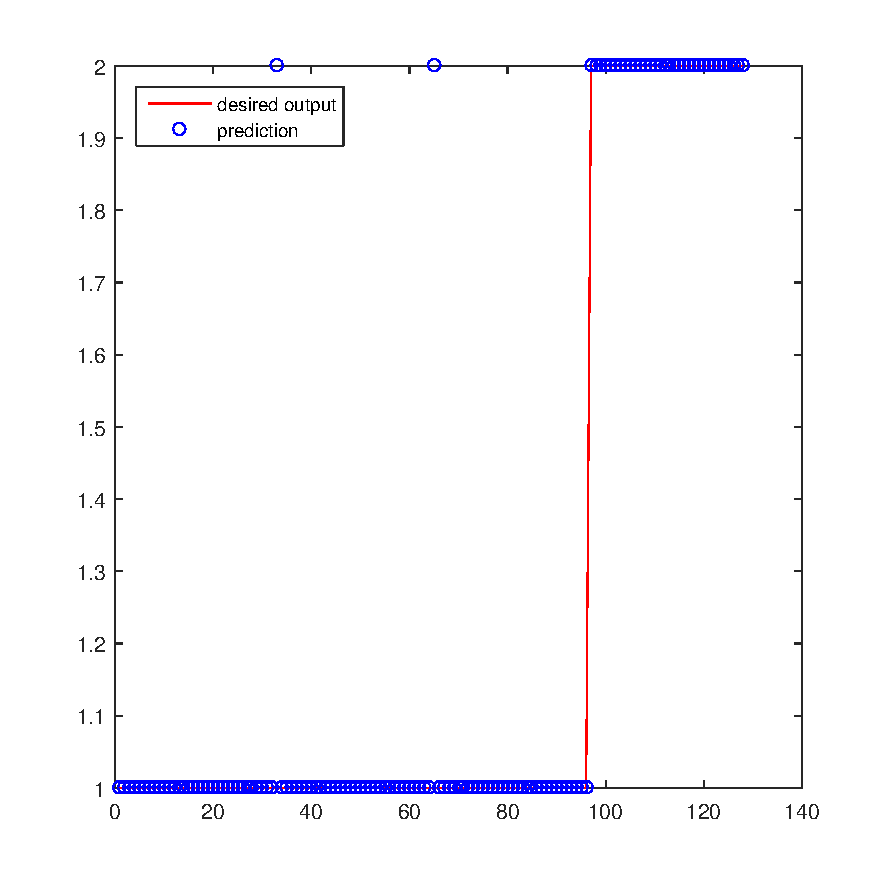
\includegraphics[scale=0.6]{breasths1}
	 		\caption{accuracy: 98.4\%} 
	 	\end{figure}
	 	\newpage
	 	\item results from toolbox 
		 	\begin{figure}[H]
	 		\centering
	 		\begin{subfigure}{.5\textwidth}
	 			\centering
	 			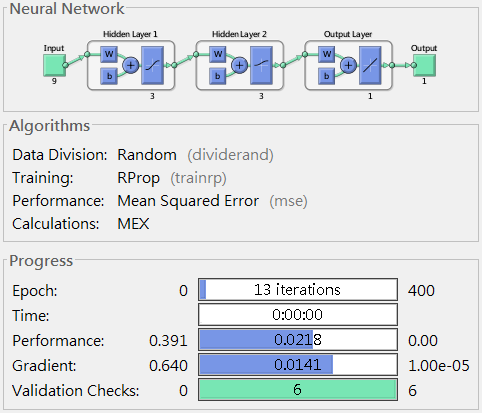
\includegraphics[width=0.92\linewidth]{RP3}
	 			\caption{RP}
	 			
	 		\end{subfigure}%
	 		\begin{subfigure}{.5\textwidth}
	 			\centering
	 			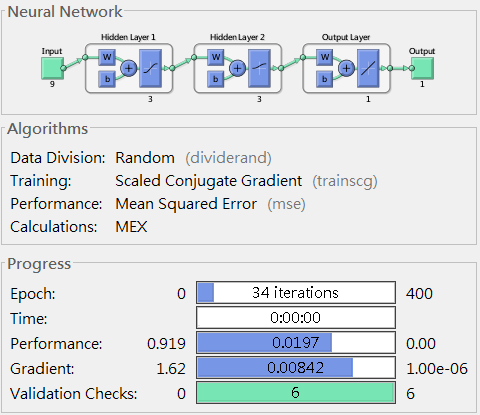
\includegraphics[width=0.92\linewidth]{SCG3}
	 			\caption{SCG}
	 			
	 		\end{subfigure}
	 		\caption{Sturctures \& Parameters}
	 		
	 	\end{figure}
	 	
	 	
	 	\begin{figure}[H]
	 		\centering
	 		\begin{subfigure}{.5\textwidth}
	 			\centering
	 			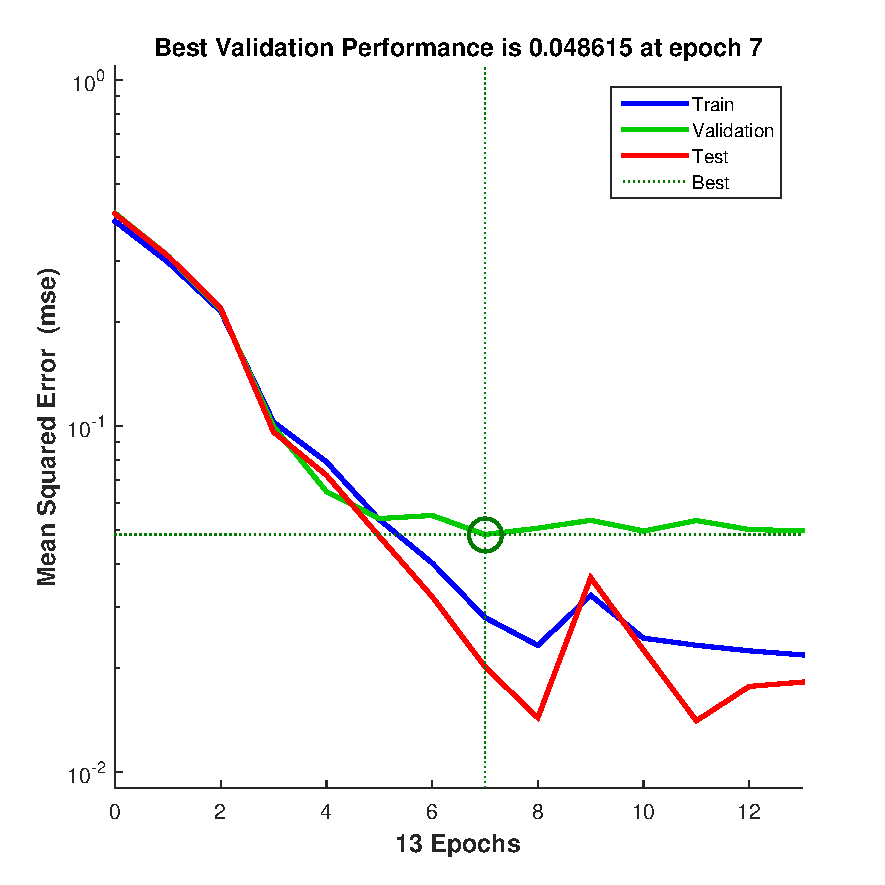
\includegraphics[width=1\linewidth]{breast_rp_per}
	 			\caption{RP}
	 			
	 		\end{subfigure}%
	 		\begin{subfigure}{.5\textwidth}
	 			\centering
	 			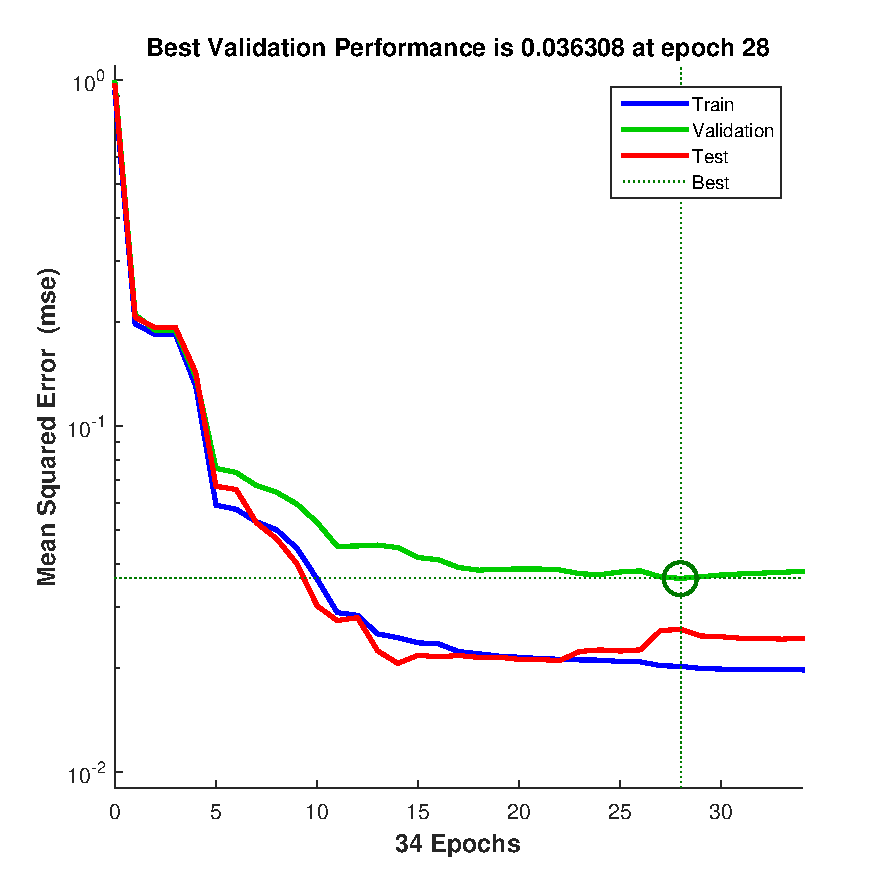
\includegraphics[width=1\linewidth]{breast_scg_per}
	 			\caption{SCG}
	 			
	 		\end{subfigure}
	 		\caption{performance}
	 		
	 	\end{figure}
	 	
	 	\begin{figure}[H]
	 		\centering
	 		\begin{subfigure}{.5\textwidth}
	 			\centering
	 			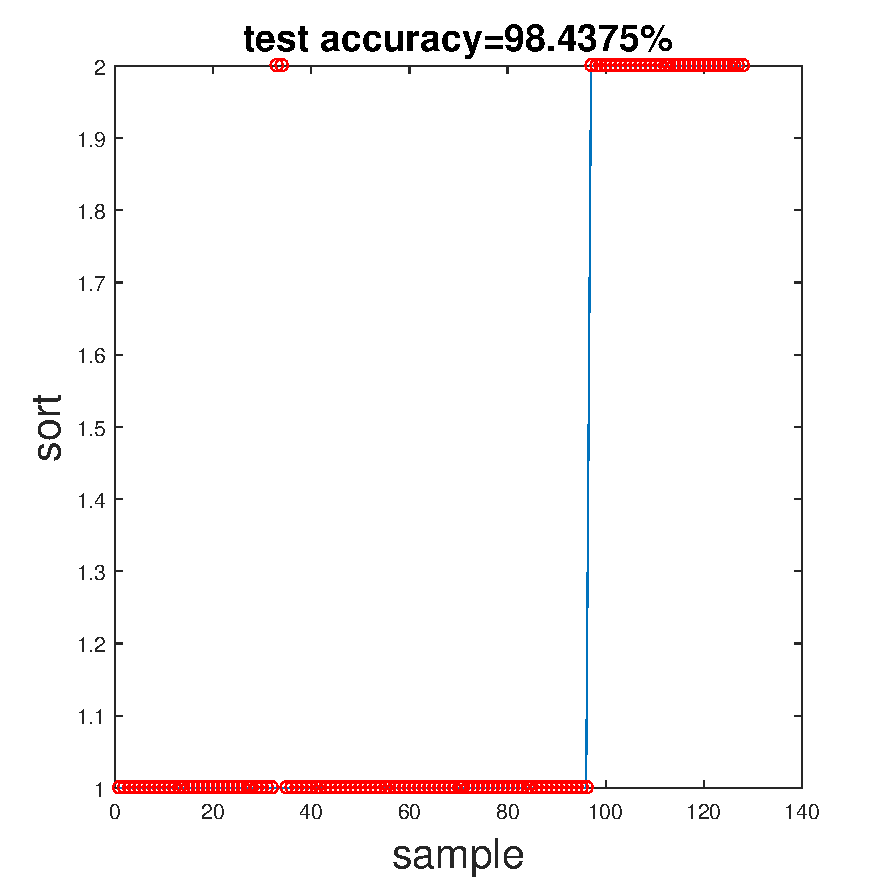
\includegraphics[width=1.05\linewidth]{breast_rp}
	 			\caption{RP}
	 			
	 		\end{subfigure}%
	 		\begin{subfigure}{.5\textwidth}
	 			\centering
	 			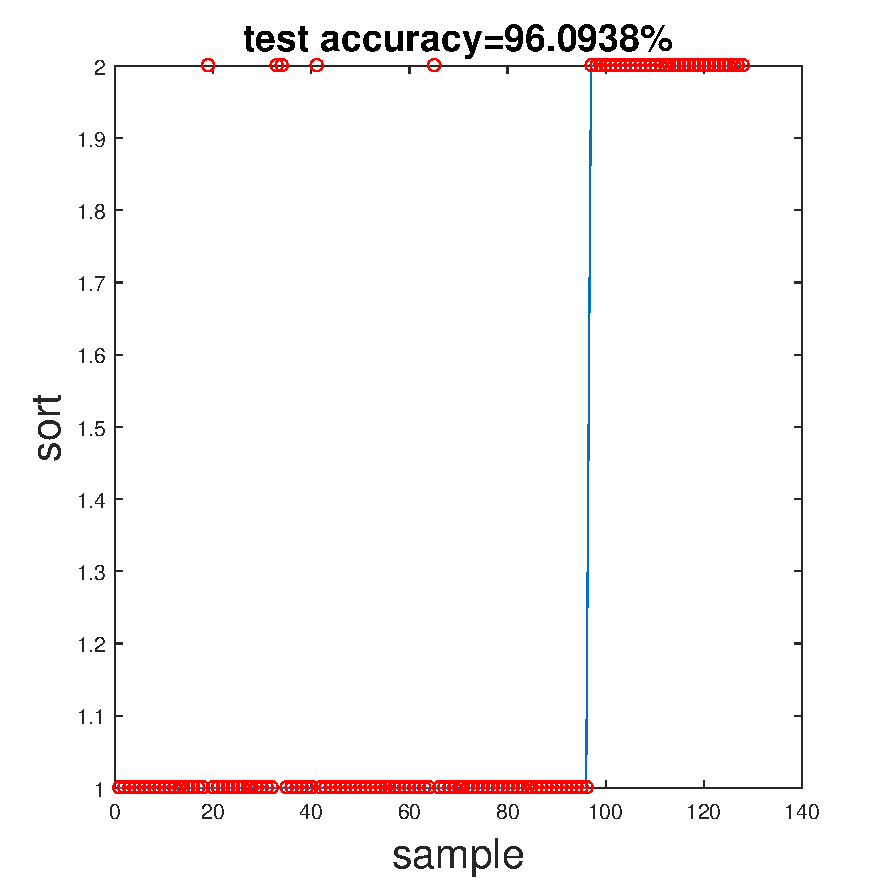
\includegraphics[width=1.05\linewidth]{breast_scg}
	 			\caption{SCG}
	 			
	 		\end{subfigure}
	 		\caption{accuracy}
	 		
	 	\end{figure}
	 	
	 	\begin{table}[H]
	 		\caption{accuracy of two algorithm} % title of Table
	 		\centering % used for centering table
	 		\begin{tabular}{c c c c c c c} % centered columns (4 columns)
	 			\hline\hline %inserts double horizontal lines
	 			algorithm & test1 & test2 & test3 & test4 &test5 & average\\ [0.5ex] % inserts table
	 			%heading
	 			\hline % inserts single horizontal line
	 			RP & 98.44\% & 94.53\% & 97.66\% & 99.22\% &98.44\% &97.66\%\\ % inserting body of the table
	 			
	 			SCG & 96.88\% & 96.88\% & 96.09\% & 96.09\% &96.88\% &96.41\%\\
	 			[0.5ex] % [1ex] adds vertical space
	 			\hline %inserts single line
	 		\end{tabular}
	 	\end{table}

	 \end{enumerate}
	 \newpage
	 
	 %% yeast
	 \item Yeast
	 
	  \begin{enumerate}
	 	\begin{table}[H]
	 		\caption{parameters of yeast} % title of Table
	 		\centering % used for centering table
	 		\begin{tabular}{c c c c c} % centered columns (4 columns)
	 			\hline\hline %inserts double horizontal lines
	 			& Epoch & Learning rate & first hidden & second hidden \\ [0.5ex] % inserts table
	 			%heading
	 			\hline % inserts single horizontal line
	 			HW2 & 500 & 0.1 & 5 & 7\\ % inserting body of the table
	 			toolbox & N/A & 0.0015 & 5 & 7\\
	 			[0.5ex] % [1ex] adds vertical space
	 			\hline %inserts single line
	 		\end{tabular}
	 		\label{table:nonlin} % is used to refer this table in the text
	 	\end{table}

	 	\item results from HW2 
	 	\\
	 	\begin{figure}[H]
	 		\centering
	 		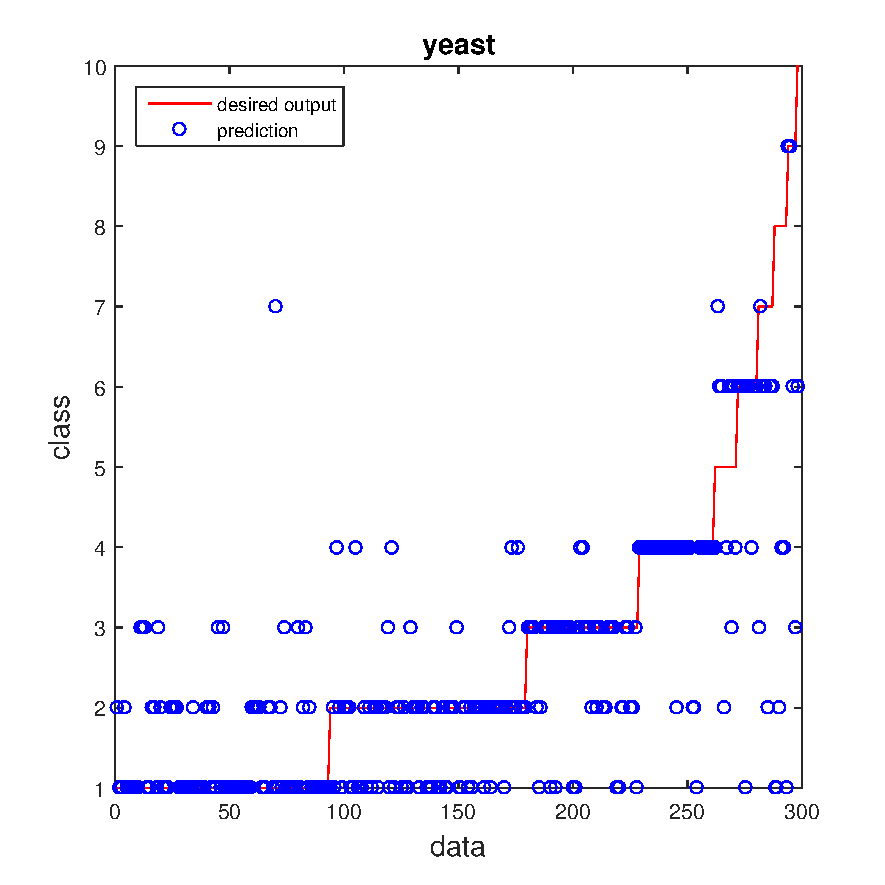
\includegraphics[scale=0.6]{yeasths2}
	 		\caption{accuracy: 58.4\%} 
	 	\end{figure}
	 	\newpage
	 	\item results from toolbox 
	 	\begin{figure}[H]
	 		\centering
	 		\begin{subfigure}{.5\textwidth}
	 			\centering
	 			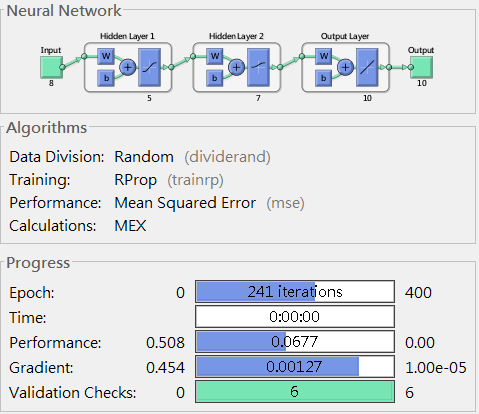
\includegraphics[width=0.92\linewidth]{RP4}
	 			\caption{RP}
	 			
	 		\end{subfigure}%
	 		\begin{subfigure}{.5\textwidth}
	 			\centering
	 			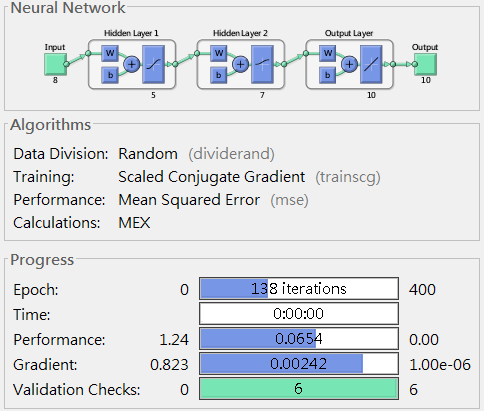
\includegraphics[width=0.92\linewidth]{SCG4}
	 			\caption{SCG}
	 			
	 		\end{subfigure}
	 		\caption{Sturctures \& Parameters}
	 		
	 	\end{figure}
	 	
	 	
	 	\begin{figure}[H]
	 		\centering
	 		\begin{subfigure}{.5\textwidth}
	 			\centering
	 			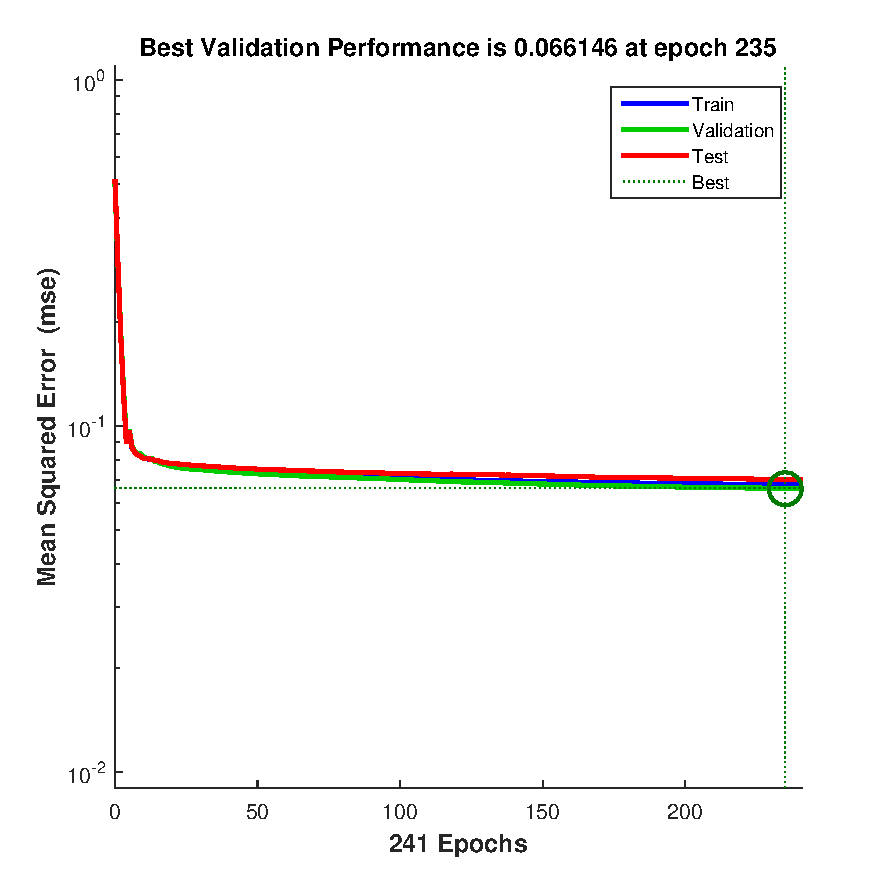
\includegraphics[width=1\linewidth]{yeast_rp_per}
	 			\caption{RP}
	 			
	 		\end{subfigure}%
	 		\begin{subfigure}{.5\textwidth}
	 			\centering
	 			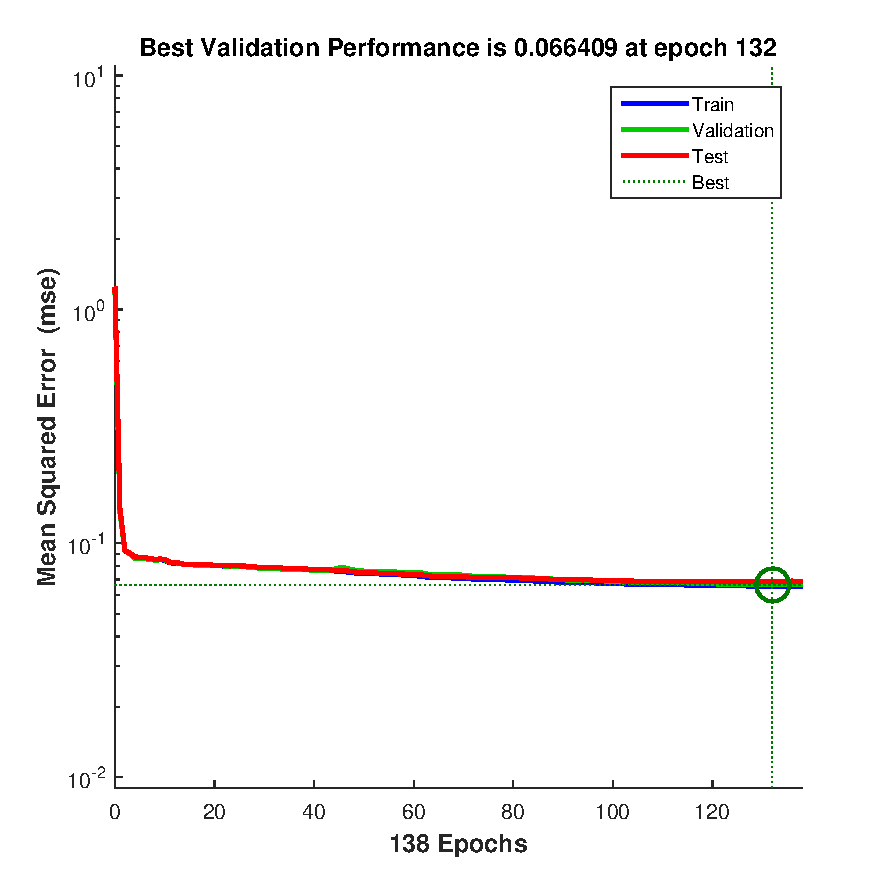
\includegraphics[width=1\linewidth]{yeast_scg_per}
	 			\caption{SCG}
	 			
	 		\end{subfigure}
	 		\caption{performance}
	 		
	 	\end{figure}
	 	
	 	\begin{figure}[H]
	 		\centering
	 		\begin{subfigure}{.5\textwidth}
	 			\centering
	 			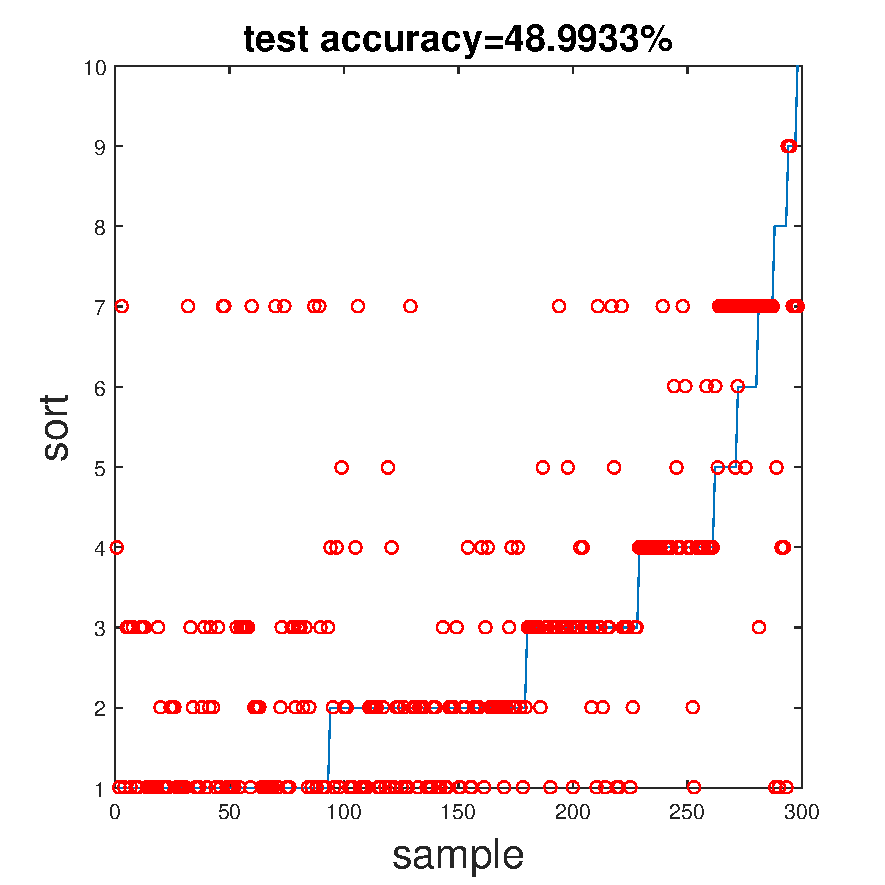
\includegraphics[width=1.05\linewidth]{yeast_rp}
	 			\caption{RP}
	 			
	 		\end{subfigure}%
	 		\begin{subfigure}{.5\textwidth}
	 			\centering
	 			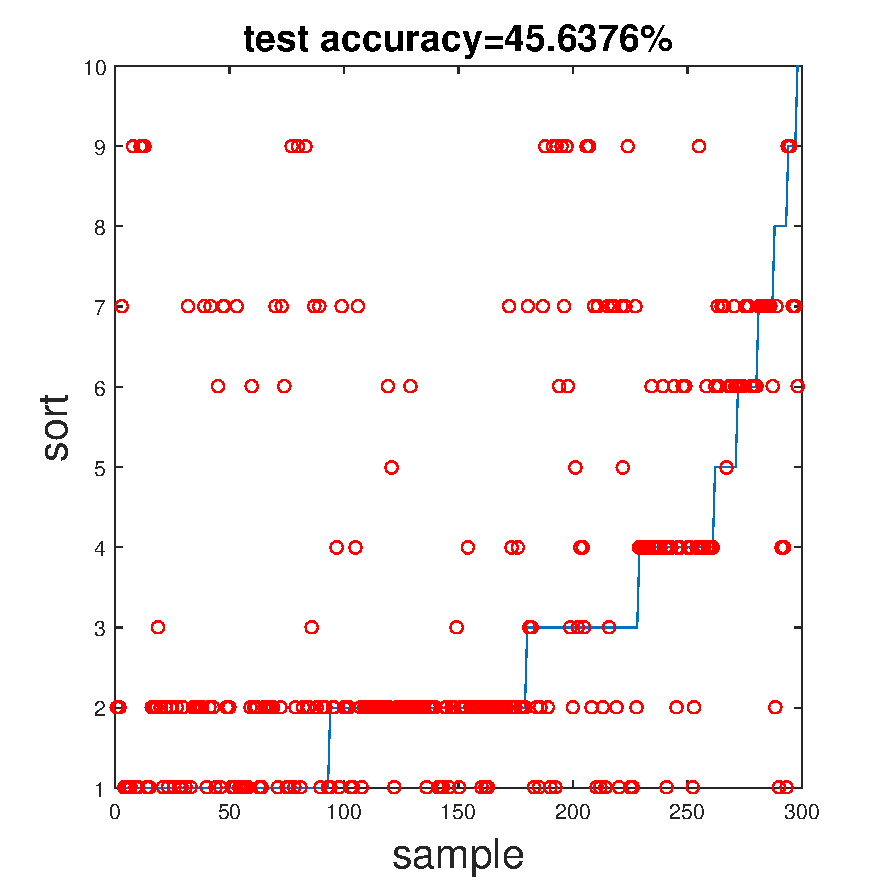
\includegraphics[width=1.05\linewidth]{yeast_scg}
	 			\caption{SCG}
	 			
	 		\end{subfigure}
	 		\caption{accuracy}
	 		
	 	\end{figure}
	 	
	 	\begin{table}[H]
	 		\caption{accuracy of two algorithm} % title of Table
	 		\centering % used for centering table
	 		\begin{tabular}{c c c c c c c} % centered columns (4 columns)
	 			\hline\hline %inserts double horizontal lines
	 			algorithm & test1 & test2 & test3 & test4 &test5 & average\\ [0.5ex] % inserts table
	 			%heading
	 			\hline % inserts single horizontal line
	 			RP & 48.99\% & 43.62\% & 45.64\% & 47.65\% &45.64\% &46.31\%\\ % inserting body of the table
	 			
	 			SCG & 45.64\% & 40.27\% & 41.95\% & 52.01\% &41.28\% &44.23\%\\
	 			[0.5ex] % [1ex] adds vertical space
	 			\hline %inserts single line
	 		\end{tabular}
	 	\end{table}

	 \end{enumerate}
	 %\newpage
	 \vspace{1cm}
	 \title{\large \bf Discussion}
	 \\
	 \setlength{\parindent}{5ex}
	 \indent
	  I use Resillent Backpropagation and Scaled Conjugate Gradient for all four data sets. I find that these two algorithms works. The two algorithms have similar accuracy for all data sets, and both can predict well. In this case, there is no such difference between two algorithms. When comparing toolbox with my code in HW2, there is still no difference more than 5\%.
	
	\end{enumerate}
	
\end{CJK}

\end{document}